\documentclass[border=10pt]{standalone}
\usepackage{tikz}
\usetikzlibrary{shapes, positioning, arrows.meta, calc}

\begin{document}
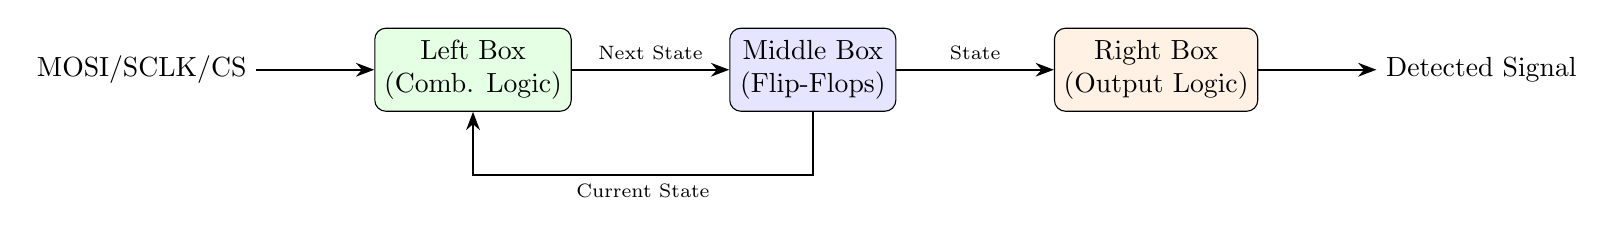
\begin{tikzpicture}[
    >=Stealth,
    node distance=2cm,
    block/.style={draw, rectangle, minimum height=3em, minimum width=6em, align=center, fill=white, rounded corners},
    input/.style={coordinate}
]

    % Nodes
    \node[block, fill=green!10] (left) {Left Box \\ (Comb. Logic)};
    \node[block, fill=blue!10, right=of left] (middle) {Middle Box \\ (Flip-Flops)};
    \node[block, fill=orange!10, right=of middle] (right) {Right Box \\ (Output Logic)};
    
    % Inputs
    \node[left=1.5cm of left] (input) {MOSI/SCLK/CS};
    \node[right=1.5cm of right] (output) {Detected Signal};

    % Connections
    \draw[->, thick] (input) -- (left);
    \draw[->, thick] (left) -- node[above, font=\scriptsize] {Next State} (middle);
    \draw[->, thick] (middle) -- node[above, font=\scriptsize] {State} (right);
    \draw[->, thick] (right) -- (output);
    
    % Feedback
    \draw[->, thick] (middle.south) -- ++(0, -0.8) coordinate(fb) -- (fb -| left.south) -- (left.south);
    \node[below, font=\scriptsize] at ($(fb)!0.5!(fb -| left.south)$) {Current State};

\end{tikzpicture}
\end{document}
